\begin{figure}[t]
\centering
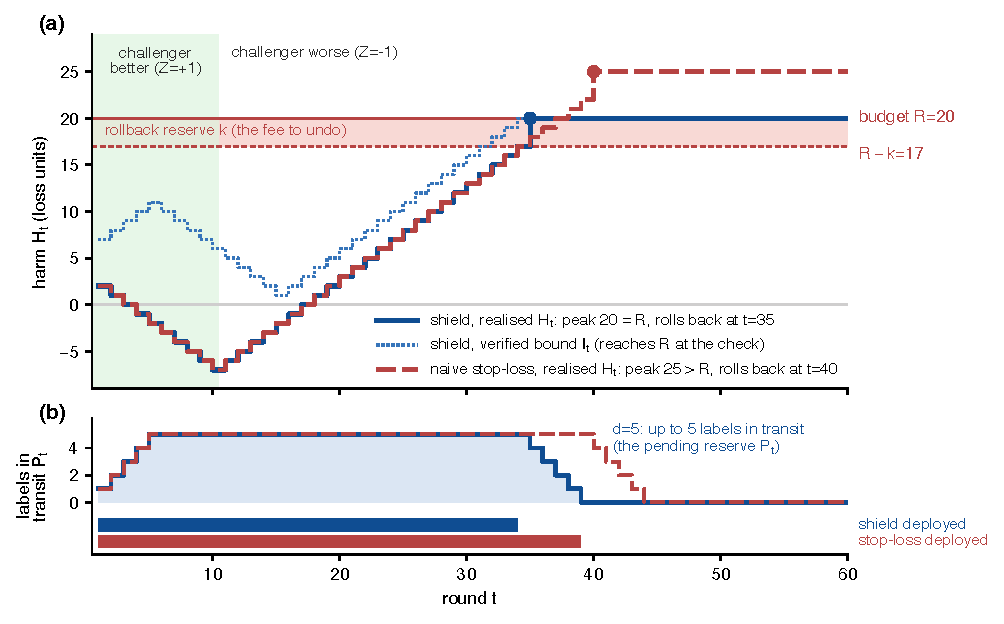
\includegraphics[width=\linewidth]{figures/fig_mechanism.pdf}
\caption{The shield stays within the budget on a tape where a naive stop-loss overshoots it. Tape: 60 rounds, every round a disagreement, the challenger better ($Z=+1$) for the first 10 rounds and worse ($Z=-1$) afterwards, label delay $d=5$, fee $k=3$, budget $R=20$, inner rule always-challenger. (a) Realised harm $H_t$ of the shield (solid) and of a stop-loss that rolls back when fees plus resolved harm exceed $R-k$ (dashed), with the shield's check (dotted; fees, rollback reserve $k$, resolved and pending harm, cf.\ $W_t$ in Section~\ref{sec:method}), evaluated after round $t$ (shaded band between $R-k$ and $R$). The shield rolls back at round 35 with peak harm exactly 20; the stop-loss, blind to the five labels in transit and to the rollback fee, rolls back at round 40 with peak harm 25. (b) Labels in transit and rounds on which each controller is deployed. Both traces are computed by running the committed code on this tape.}
\label{fig:mechanism}
\end{figure}
